\chapter{RESULTADOS E DISCUSSÃO}\label{sec:resultados}

Nesta seção, apresentam-se os resultados da campanha de treinamento e a resposta às três perguntas definidas na \autoref{sec:analise}. O RMSE é sempre o da simulação livre.

\section{Campanha de treinamento e escala do erro}\label{sec:campanha}

Com as tentativas de cada braço executadas em paralelo \pendente{descrever a máquina e o número de processos simultâneos}, cada treinamento 5×2 levou cerca de 13,6~h (mediana) e cada treinamento 5×3, cerca de 23,1~h. A terceira saída aumenta em cerca de 70\% o custo de cada execução, pois cada indivíduo passa a ter 21 genes em vez de 14 e a avaliação de cada um envolve três saídas realimentadas. Além disso, 2 dos 30 treinamentos 5×3 (6,7\%) foram reprovados na validação, contra nenhum dos 30 do braço 5×2. Essa diferença de robustez não entra nos testes estatísticos, que usam apenas os modelos aprovados.

A simulação livre divergiu em apenas um par modelo × pista em cada braço, ambos na pista de treino, a mais longa (cerca de 210~s, ou 42 mil passos recursivos). Nenhum modelo divergiu nas pistas de teste; assim, as comparações das seções seguintes envolvem 30 modelos 5×2 e 28 modelos 5×3 em cada pista de teste.

As duas últimas colunas da \autoref{tab:pistas} dão a escala do erro de $\beta$ na ausência de qualquer modelo. Estimar $\hat\beta = 0$ resulta em RMSE entre 2,24° (Wang 3.1) e 4,52° (Wang 8.1) nas pistas de teste, e usar a média de $\beta$ do treino reduz pouco esse valor. A Wang 8.1 é a pista com manobras mais severas ($\sigma_\beta = 4{,}21^\circ$), o que antecipa que ela será a mais difícil para todos os estimadores.

\section{Referência cinemática e modelos da Iniciação Científica}\label{sec:referencias}

A \autoref{tab:referencias_beta} compara o estimador cinemático e os modelos de referência da IC com a mediana dos modelos da campanha. Os modelos T48 e T19 da IC foram reavaliados e reproduziram os valores publicados naquela pesquisa (RMSE médio das velocidades de 0,2121~m/s e 0,2240~m/s, respectivamente, nas quatro pistas usadas pela IC).

\begin{table}[htbp]
    \centering
    \caption{RMSE de $\beta$ (graus) do estimador cinemático, dos modelos de referência da IC (T48 e T19, $\beta$ pós-calculado) e mediana dos modelos da campanha.}
    \label{tab:referencias_beta}
    \footnotesize
    \begin{tabular}{lccccc}
        \toprule
        \textbf{Pista} & \textbf{Cinemático} & \textbf{IC T48} & \textbf{IC T19} & \textbf{5×2 + atan2} & \textbf{5×3, saída 3} \\
        \midrule
        Wang 2.1 (treino) & 22,395 & 1,506 & 1,624 & 1,647 & 1,527 \\
        Wang 2.2 (validação) & 2,076 & 0,448 & 0,708 & 0,609 & 0,776 \\
        Wang 3.1 (teste A) & 3,213 & 0,700 & 0,952 & 0,979 & 0,882 \\
        Wang 8.1 (teste B) & 2,899 & 1,334 & 1,367 & 1,434 & 1,482 \\
        Wang 3.2 (teste C) & 1,179 & 1,523 & 1,447 & 1,738 & 1,098 \\
        \bottomrule
    \end{tabular}
    \par\footnotesize Nota: cinemático: integração de $\dot\beta = a_y/\hat v_x + \dot\psi$ com $\hat v_x$ proporcional à velocidade da roda traseira, sem realimentação de medição; sinal do termo de guinada escolhido na pista de treino. T48 e T19 foram selecionados pela IC olhando as pistas Wang 2.1 a 8.1.
    \fonte{Elaboração própria.}
\end{table}


O estimador cinemático, que apenas integra a \autoref{eq:beta_cinematica}, tem RMSE de 22,4° na pista de treino, de 210~s, e entre 1,2° e 3,2° nas demais, mais curtas. A pista de treino é a mais longa, mas também contém trechos de baixa velocidade (\autoref{fig:sinais_wang21}f), nos quais o termo $a_y/v_x$ é mal condicionado. Portanto, a deriva observada não pode ser atribuída apenas à duração do ensaio, e os dois efeitos não foram separados. Com exceção da Wang 3.2, em que o estimador cinemático (1,179°) fica abaixo dos modelos 5×2 (mediana de 1,738°) e dos modelos T48 e T19 da IC (1,523° e 1,447°) e próximo da mediana dos modelos 5×3 (1,098°), os modelos MGGP têm RMSE bem menor que o cinemático. Isso indica que os modelos MGGP incorporam alguma forma de correção da deriva da integração; a natureza dessa correção não foi isolada (\autoref{sec:limitacoes}). Esse estimador é uma linha de base simples, sem correção por medições externas, e não representa o desempenho de estimadores cinemáticos com fusão sensorial descritos na literatura.

Na \autoref{tab:referencias_beta}, o sinal do termo de guinada do estimador cinemático foi escolhido na pista de treino e difere do sinal da \autoref{eq:beta_cinematica}. A diferença decorre da convenção de eixos do sensor de taxa de guinada, que nos dados tem sinal oposto ao de $a_y$ nas curvas: no ensaio de treino, a correlação entre $a_y$ e $v_x\dot\psi$ é de $-0{,}87$. Com esse sinal, a forma $\dot\beta \approx a_y/v_x + \dot\psi$ reproduz a derivada numérica de $\beta$ com erro de 3,7~graus/s (para $v_x > 3$~m/s), contra 21,6~graus/s com o sinal da \autoref{eq:beta_cinematica}.

Os modelos T48 e T19 da IC obtêm valores próximos ou melhores que os da mediana da campanha, inclusive na Wang 3.2, que não havia sido usada naquela pesquisa. Isso era esperado: são modelos 5×2 da mesma configuração, mas foram selecionados pela IC por terem o menor erro entre dez execuções, observando justamente as pistas de validação e de teste A e B. A mediana da campanha, ao contrário, representa um modelo típico, sem seleção.

Como linha de base linear, ajustou-se por mínimos quadrados, na pista de treino, um modelo com as mesmas entradas e os mesmos atrasos dos modelos MGGP (\autoref{tab:linear}). A versão com realimentação das saídas divergiu na simulação livre, já na pista de treino. A versão sem realimentação, que usa apenas as entradas atrasadas, é estável, mas seu RMSE de $\beta$ nas pistas de teste (entre 1,8° e 4,0°) é maior do que a mediana dos modelos MGGP (entre 0,9° e 1,7°) em todas as pistas; o de $v_x$ (0,30 a 0,48~m/s) também supera o dos modelos MGGP 5×2 (0,16~m/s na Wang 8.1 e 0,10~m/s na Wang 3.2).

\begin{table}[htbp]
    \centering
    \caption{RMSE de $\beta$ (graus) de um modelo linear de mesmas entradas e atrasos, sem realimentação das saídas, e mediana dos modelos MGGP.}
    \label{tab:linear}
    \footnotesize
    \begin{tabular}{lcccc}
        \toprule
        \textbf{Pista} & \textbf{Linear 5×2 + atan2} & \textbf{Linear 5×3, saída 3} & \textbf{MGGP 5×2 + atan2} & \textbf{MGGP 5×3, saída 3} \\
        \midrule
        Wang 2.1 (treino) & 2,093 & 1,991 & 1,647 & 1,527 \\
        Wang 2.2 (validação) & 2,144 & 2,040 & 0,609 & 0,776 \\
        Wang 3.1 (teste A) & 1,868 & 1,807 & 0,979 & 0,882 \\
        Wang 8.1 (teste B) & 3,812 & 3,996 & 1,434 & 1,482 \\
        Wang 3.2 (teste C) & 2,105 & 2,052 & 1,738 & 1,098 \\
        \bottomrule
    \end{tabular}
    \par\footnotesize Nota: o modelo linear usa as entradas nos atrasos $[1, 2, 5, 10, 25, 50]$ ajustado por mínimos quadrados na pista de treino; a versão com realimentação das saídas divergiu na simulação livre.
    \fonte{Elaboração própria.}
\end{table}


Como ponto de comparação com a literatura, \citeonline{prieto2020} estimam o ângulo de deriva de uma van (Mercedes Sprinter) com uma rede neural profunda alimentada por acelerações, taxa de rolagem, taxa de guinada, ângulo de esterçamento e velocidade longitudinal. Em ensaio real em pista, com manobras em rotatórias e em slalom, os autores reportam RMSE de 1,40° e erro máximo de 6,36°; em simulação, o RMSE é de 0,03° ou menos. O RMSE de 0,9° a 1,7° deste trabalho está na mesma ordem de grandeza do ensaio real daquele estudo, mas a comparação é apenas indicativa: o veículo, as manobras, o conjunto de sensores (o ângulo de esterçamento não é entrada aqui) e a referência são diferentes. \pendente{incluir ao menos mais um trabalho com ensaio experimental e RMSE de $\beta$ em graus}

\section{Qualidade do ângulo de deriva}\label{sec:q1}

A \autoref{fig:rmse_beta} e a \autoref{tab:resumo_beta} apresentam a distribuição do RMSE de $\beta$ entre os modelos, por pista e por variante, e a \autoref{tab:testes} reúne os testes confirmatórios.

\begin{figure}[htbp]
    \centering
    \caption{Distribuição do RMSE de $\beta$ entre os modelos, por pista e por variante. A linha tracejada é o RMSE de $\hat\beta = 0$.}
    \label{fig:rmse_beta}
    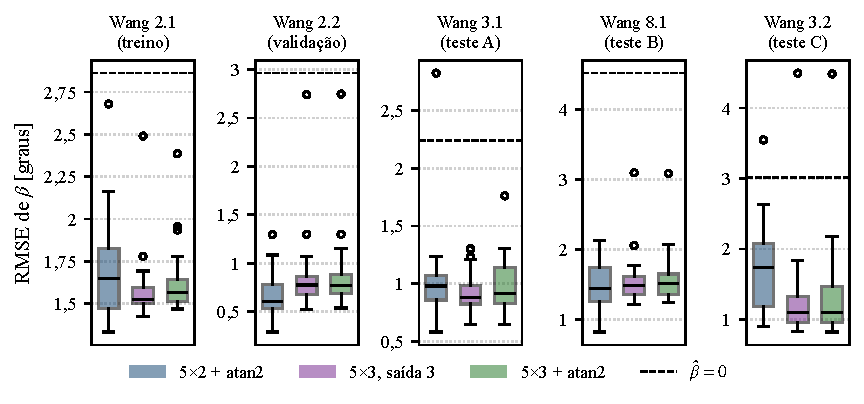
\includegraphics[width=\textwidth]{figuras/rmse_beta_boxplot.pdf}
    \fonte{Elaboração própria.}
\end{figure}

\begin{table}[htbp]
    \centering
    \caption{RMSE de $\beta$ (graus) por pista e variante: mediana, intervalo interquartil, média e desvio-padrão entre os modelos.}
    \label{tab:resumo_beta}
    \footnotesize
    \begin{tabular}{llrcccc}
        \toprule
        \textbf{Pista} & \textbf{Variante} & $n$ & \textbf{Mediana} & \textbf{[Q1; Q3]} & \textbf{Média} & \textbf{DP} \\
        \midrule
        Wang 2.1 (treino) & 5×2 + atan2 & 29 & 1,647 & [1,469; 1,825] & 1,683 & 0,300 \\
         & 5×3, saída 3 & 27 & 1,527 & [1,499; 1,593] & 1,582 & 0,197 \\
         & 5×3 + atan2 & 27 & 1,564 & [1,512; 1,641] & 1,626 & 0,200 \\
        Wang 2.2 (validação) & 5×2 + atan2 & 30 & 0,609 & [0,531; 0,784] & 0,665 & 0,216 \\
         & 5×3, saída 3 & 28 & 0,776 & [0,679; 0,859] & 0,853 & 0,403 \\
         & 5×3 + atan2 & 28 & 0,766 & [0,684; 0,880] & 0,864 & 0,408 \\
        Wang 3.1 (teste A) & 5×2 + atan2 & 30 & 0,979 & [0,858; 1,070] & 1,012 & 0,385 \\
         & 5×3, saída 3 & 28 & 0,882 & [0,823; 0,983] & 0,928 & 0,180 \\
         & 5×3 + atan2 & 28 & 0,917 & [0,826; 1,143] & 0,990 & 0,246 \\
        Wang 8.1 (teste B) & 5×2 + atan2 & 30 & 1,434 & [1,253; 1,739] & 1,507 & 0,339 \\
         & 5×3, saída 3 & 28 & 1,482 & [1,357; 1,608] & 1,541 & 0,352 \\
         & 5×3 + atan2 & 28 & 1,506 & [1,356; 1,647] & 1,574 & 0,360 \\
        Wang 3.2 (teste C) & 5×2 + atan2 & 30 & 1,738 & [1,183; 2,076] & 1,758 & 0,603 \\
         & 5×3, saída 3 & 28 & 1,098 & [0,960; 1,324] & 1,274 & 0,679 \\
         & 5×3 + atan2 & 28 & 1,099 & [0,961; 1,460] & 1,350 & 0,718 \\
        \bottomrule
    \end{tabular}
    \fonte{Elaboração própria.}
\end{table}


\begin{table}[htbp]
    \centering
    \caption{Testes confirmatórios nas pistas de teste: diferença de medianas com IC95\% \textit{bootstrap}, tamanho de efeito e valor-p corrigido por Holm em cada família.}
    \label{tab:testes}
    \scriptsize
    \begin{tabular}{lllcccrc}
        \toprule
        \textbf{Q} & \textbf{Comparação} & \textbf{Pista} & $n_1/n_2$ & \textbf{Dif.} & \textbf{IC95\%} & \textbf{Efeito} & \textbf{p (Holm)} \\
        \midrule
        Q1 & $\beta$: 5×3 atan2 $-$ 5×2 & Wang 3.1 & 28/30 & $-$0,062 & [$-$0,175; 0,128] & $-$0,00 & 1,0000 \\
        Q1 & $\beta$: 5×3 atan2 $-$ 5×2 & Wang 8.1 & 28/30 & 0,072 & [$-$0,158; 0,217] & 0,10 & 1,0000 \\
        Q1 & $\beta$: 5×3 atan2 $-$ 5×2 & Wang 3.2 & 28/30 & $-$0,639 & [$-$0,904; $-$0,291] & $-$0,50 & 0,0056 \\
        Q1 & $\beta$: 5×3 saída 3 $-$ 5×2 & Wang 3.1 & 28/30 & $-$0,097 & [$-$0,199; 0,026] & $-$0,15 & 1,0000 \\
        Q1 & $\beta$: 5×3 saída 3 $-$ 5×2 & Wang 8.1 & 28/30 & 0,048 & [$-$0,171; 0,168] & 0,06 & 1,0000 \\
        Q1 & $\beta$: 5×3 saída 3 $-$ 5×2 & Wang 3.2 & 28/30 & $-$0,641 & [$-$0,903; $-$0,362] & $-$0,59 & 0,0007 \\
        Q2 & $v_x$: 5×3 $-$ 5×2 & Wang 3.1 & 28/30 & 0,028 & [$-$0,087; 0,150] & 0,11 & 0,4887 \\
        Q2 & $v_x$: 5×3 $-$ 5×2 & Wang 8.1 & 28/30 & 0,093 & [0,026; 0,219] & 0,59 & 0,0006 \\
        Q2 & $v_x$: 5×3 $-$ 5×2 & Wang 3.2 & 28/30 & 0,256 & [0,137; 0,295] & 0,84 & $<$0,0001 \\
        Q2 & $v_y$: 5×3 $-$ 5×2 & Wang 3.1 & 28/30 & 0,033 & [$-$0,007; 0,062] & 0,34 & 0,1022 \\
        Q2 & $v_y$: 5×3 $-$ 5×2 & Wang 8.1 & 28/30 & 0,022 & [$-$0,035; 0,070] & 0,18 & 0,4678 \\
        Q2 & $v_y$: 5×3 $-$ 5×2 & Wang 3.2 & 28/30 & $-$0,068 & [$-$0,121; $-$0,020] & $-$0,24 & 0,3647 \\
        Q3 & $\beta$: saída 3 $-$ atan2 (5×3) & Wang 3.1 & 28/28 & $-$0,004 & [$-$0,020; $-$0,002] & 0,89 & 0,0002 \\
        Q3 & $\beta$: saída 3 $-$ atan2 (5×3) & Wang 8.1 & 28/28 & $-$0,017 & [$-$0,027; $-$0,007] & 0,71 & 0,1128 \\
        Q3 & $\beta$: saída 3 $-$ atan2 (5×3) & Wang 3.2 & 28/28 & $-$0,002 & [$-$0,009; 0,001] & 0,68 & 0,2545 \\
        \bottomrule
    \end{tabular}
    \par\footnotesize Nota: Q1 e Q2: Mann--Whitney, efeito = $\delta$ de Cliff (negativo: o 5×3 erra menos). Q3: Wilcoxon pareado por modelo, diferença = mediana das diferenças, efeito = fração de modelos em que a saída 3 erra menos. RMSE de $\beta$ em graus; de $v_x$, $v_y$ em m/s.
    \fonte{Elaboração própria.}
\end{table}


Em duas das três pistas de teste, Wang 3.1 e Wang 8.1, não há diferença significativa entre o ângulo obtido pelos modelos 5×3 (pela saída evoluída ou pelo $\operatorname{atan2}$ das velocidades) e o ângulo pós-calculado dos modelos 5×2. As diferenças de medianas ficam abaixo de 0,1° e os intervalos de confiança de 95\% incluem o zero, indo de cerca de $-0{,}2^\circ$ a $+0{,}2^\circ$. Os dados, portanto, não indicam diferença, mas também não permitem excluir diferenças dessa ordem, que correspondem a 15 a 20\% do RMSE mediano.

Na Wang 3.2, ao contrário, os modelos 5×3 erram menos: a mediana do RMSE cai de 1,74° para 1,10°, com $\delta$ de Cliff de $-0{,}59$ (efeito grande) e $p = 0{,}0007$ após a correção de Holm. Esse resultado vem de uma única pista e deve ser lido com cautela. Como descrito na \autoref{sec:proveniencia}, a velocidade lateral de referência das três pistas de teste está deslocada em relação ao valor implícito no ângulo de deriva bruto, o que pode favorecer ou prejudicar um braço conforme o viés de cada modelo.

Para medir essa sensibilidade, os modelos já treinados foram reavaliados, sem retreinamento, contra uma referência em que o deslocamento de $v_y$ (0,31, 0,37 e 0,31~m/s nas três pistas de teste) é subtraído antes do cálculo de $\beta$ (\autoref{tab:reavaliacao}). A comparação se inverte: com a referência corrigida, os modelos 5×2 erram menos do que os 5×3 nas três pistas. Para a saída evoluída, a diferença de medianas (5×3 menos 5×2) é de $+0{,}16^\circ$ na Wang 3.1, $+0{,}45^\circ$ na Wang 8.1 e $+0{,}28^\circ$ na Wang 3.2, com $\delta$ de Cliff de cerca de $+0{,}55$ e $p \le 0{,}002$ após a correção de Holm sobre as seis comparações. O viés, que era negativo para todos os estimadores em relação à referência original (entre $-0{,}6^\circ$ e $-1{,}4^\circ$), torna-se positivo em relação à corrigida (entre $+0{,}2^\circ$ e $+0{,}9^\circ$): os modelos ficam entre as duas referências. Removendo o viés, o RMSE contra a referência original é menor para o 5×3 na Wang 3.2 (0,77° contra 0,99°), praticamente igual na Wang 3.1 (0,65° contra 0,67°) e maior na Wang 8.1 (1,23° contra 0,82°); contra a referência corrigida, o 5×2 é melhor nas três. Portanto, a vantagem do 5×3 na Wang 3.2 não resiste à troca de referência, e os dados não permitem dizer qual das duas é a correta.

\begin{table}[htbp]
    \centering
    \caption{RMSE de $\beta$ (graus) nas pistas de teste, mediana entre modelos, contra a referência original e contra a referência com o deslocamento de $v_y$ removido; com e sem o viés.}
    \label{tab:reavaliacao}
    \small
    \begin{tabular}{llcccc}
        \toprule
        \textbf{Pista} & \textbf{Variante} & \multicolumn{2}{c}{\textbf{Referência original}} & \multicolumn{2}{c}{\textbf{Referência corrigida}} \\ & & RMSE & RMSE sem viés & RMSE & RMSE sem viés \\
        \midrule
        Wang 3.1 (teste A) & 5×2 + atan2 & 0,979 & 0,673 & 0,909 & 0,683 \\
         & 5×3, saída 3 & 0,882 & 0,645 & 1,071 & 0,861 \\
         & 5×3 + atan2 & 0,917 & 0,671 & 1,054 & 0,843 \\
        Wang 8.1 (teste B) & 5×2 + atan2 & 1,434 & 0,815 & 1,093 & 0,924 \\
         & 5×3, saída 3 & 1,482 & 1,233 & 1,539 & 1,283 \\
         & 5×3 + atan2 & 1,506 & 1,272 & 1,532 & 1,297 \\
        Wang 3.2 (teste C) & 5×2 + atan2 & 1,738 & 0,991 & 0,830 & 0,565 \\
         & 5×3, saída 3 & 1,098 & 0,773 & 1,108 & 0,697 \\
         & 5×3 + atan2 & 1,099 & 0,773 & 1,082 & 0,687 \\
        \bottomrule
    \end{tabular}
    \par\footnotesize Nota: deslocamentos de $v_y$ removidos: 0,31~m/s (Wang 3.1), 0,37~m/s (Wang 8.1) e 0,31~m/s (Wang 3.2).
    \fonte{Elaboração própria.}
\end{table}


Nas pistas exploratórias, o quadro é misto. Na Wang 2.2, os modelos 5×2 têm menor mediana (0,609° contra 0,776°); na pista de treino, os modelos 5×3 têm menor mediana (1,527° contra 1,647°) e menor dispersão. O critério de aprovação (RMSE finito, positivo e menor que 100) elimina apenas modelos divergentes e, portanto, introduz pouca seleção na Wang 2.2; a pista foi mantida como exploratória por ter participado desse critério. O resultado nela vai contra a ideia de que o 5×3 é sistematicamente melhor.

Considerando as cinco pistas, a mediana do RMSE de $\beta$ da saída evoluída é menor que a do 5×2 em três (Wang 2.1, 3.1 e 3.2) e maior em duas (Wang 2.2 e 8.1). Entre elas, apenas a diferença da Wang 3.2 é significativa nos testes confirmatórios.

A \autoref{tab:resumo_beta} mostra ainda que, em todas as pistas de teste, o intervalo interquartil do RMSE de $\beta$ é menor para a saída evoluída do que para o ângulo pós-calculado dos modelos 5×2 (na Wang 8.1, por exemplo, 0,25° contra 0,49°). O desvio-padrão, sensível a poucos modelos ruins, não acompanha esse padrão nas pistas Wang 8.1 e Wang 3.2, e a homogeneidade entre execuções não foi objeto de teste do plano de análise. Trata-se, portanto, de uma observação descritiva.

Na \autoref{tab:testes}, alguns intervalos de confiança excluem o zero enquanto o valor-p corrigido não é significativo (Q3 na Wang 8.1; $v_y$ na Wang 3.2). Isso pode ocorrer porque o intervalo é obtido por \textit{bootstrap} da diferença de medianas (ou da mediana das diferenças), enquanto o valor-p vem de um teste de postos corrigido por Holm; as duas medidas respondem a perguntas diferentes e a correção para múltiplas comparações reduz o poder.

\section{Efeito sobre as velocidades}\label{sec:q2}

A \autoref{fig:rmse_vel} e a \autoref{tab:resumo_vel} mostram o efeito da terceira saída sobre as estimativas de velocidade.

\begin{figure}[htbp]
    \centering
    \caption{Distribuição do RMSE de $v_x$ e de $v_y$ entre os modelos, por pista e por braço.}
    \label{fig:rmse_vel}
    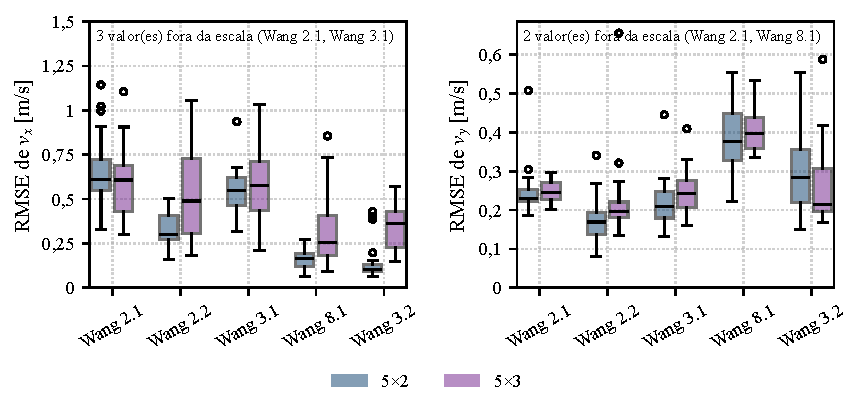
\includegraphics[width=\textwidth]{figuras/rmse_vxvy_boxplot.pdf}
    \fonte{Elaboração própria.}
\end{figure}

\begin{table}[htbp]
    \centering
    \caption{RMSE de $v_x$ e $v_y$ (m/s) por pista e braço: mediana e intervalo interquartil entre os modelos.}
    \label{tab:resumo_vel}
    \footnotesize
    \begin{tabular}{llrcccc}
        \toprule
        \textbf{Pista} & \textbf{Braço} & $n$ & \multicolumn{2}{c}{$v_x$} & \multicolumn{2}{c}{$v_y$} \\
        \midrule
        Wang 2.1 (treino) & 5×2 & 29 & 0,610 & [0,547; 0,723] & 0,231 & [0,221; 0,253] \\
         & 5×3 & 27 & 0,607 & [0,430; 0,690] & 0,245 & [0,226; 0,270] \\
        Wang 2.2 (validação) & 5×2 & 30 & 0,299 & [0,272; 0,405] & 0,169 & [0,138; 0,194] \\
         & 5×3 & 28 & 0,489 & [0,306; 0,729] & 0,195 & [0,180; 0,221] \\
        Wang 3.1 (teste A) & 5×2 & 30 & 0,550 & [0,465; 0,623] & 0,209 & [0,180; 0,248] \\
         & 5×3 & 28 & 0,579 & [0,434; 0,712] & 0,242 & [0,207; 0,277] \\
        Wang 8.1 (teste B) & 5×2 & 30 & 0,162 & [0,121; 0,191] & 0,376 & [0,327; 0,448] \\
         & 5×3 & 28 & 0,255 & [0,180; 0,405] & 0,397 & [0,358; 0,439] \\
        Wang 3.2 (teste C) & 5×2 & 30 & 0,104 & [0,092; 0,130] & 0,283 & [0,219; 0,356] \\
         & 5×3 & 28 & 0,359 & [0,228; 0,428] & 0,215 & [0,196; 0,307] \\
        \bottomrule
    \end{tabular}
    \fonte{Elaboração própria.}
\end{table}


A inclusão de $\beta$ piora a estimativa de $v_x$: nas pistas Wang 8.1 e Wang 3.2, a mediana do RMSE de $v_x$ passa de 0,16 para 0,26~m/s e de 0,10 para 0,36~m/s, respectivamente, com efeitos grandes ($\delta = 0{,}59$ e $0{,}84$) e significativos. Na estimativa de $v_y$, nenhuma diferença é significativa após a correção; a tendência é de leve piora na Wang 3.1 e de leve melhora na Wang 3.2. Esse resultado é coerente com a forma como o MGGP distribui o esforço: com a aptidão definida como a média simples dos três RMSE, e com o erro de $\beta$ em graus da mesma ordem dos erros das velocidades em m/s, o terceiro objetivo disputa com $v_x$ e $v_y$ o mesmo número de gerações e uma estrutura de indivíduo mais complexa.

\section{Saída evoluída e ângulo pós-calculado}\label{sec:q3}

Dentro de um mesmo modelo 5×3, a saída evoluída de $\beta$ e o ângulo calculado a partir das velocidades do próprio modelo são praticamente equivalentes. A mediana das diferenças vai de 0,002° a 0,017° (\autoref{tab:testes}); a saída evoluída é ligeiramente melhor na maioria dos modelos --- em 89\% deles na Wang 3.1, onde a diferença é significativa ---, mas a diferença é desprezível na prática. Isso sugere que a diferença observada na Wang 3.2 não vem de a saída $\beta$ ser mais precisa do que as velocidades do mesmo modelo, mas de os modelos 5×3 serem diferentes dos 5×2. Como a diferença em $v_y$ não foi significativa (\autoref{tab:testes}), o mecanismo dessa diferença não pôde ser identificado com os dados disponíveis.

\section{Erro por regime e simulação livre}\label{sec:regime}

Agrupando as pistas de teste, o RMSE de $\beta$ foi calculado por quartil de $|\beta|$ e de $v_x$ de cada pista (\autoref{tab:regime}). Por $|\beta|$, a variante A apresenta erro mediano entre 1,15° e 1,39°, e a saída evoluída do 5×3, entre 1,04° e 1,15°, sem tendência clara entre os quartis. Por $v_x$, o comportamento se inverte: no quartil de menor velocidade, a saída evoluída tem erro mediano de 1,03°, contra 1,37° da variante A; no quartil de maior velocidade, a variante A é melhor (0,68° contra 0,87°). O resultado é compatível com a \autoref{sec:angulo_deriva}: o $\operatorname{atan2}$ das velocidades estimadas amplifica o erro de $\hat v_y$ quando $v_x$ é baixo, e a saída evoluída, que não divide por $v_x$, é menos sensível a esse regime. A variante B\textsubscript{atan2} fica entre as duas, o que sugere que parte do ganho do 5×3 em baixa velocidade vem da forma como esses modelos estimam a própria $v_y$.

\begin{table}[htbp]
    \centering
    \caption{RMSE de $\beta$ (graus) por quartil de $|\beta|$ e de $v_x$ de cada pista: mediana entre modelos e pistas de teste.}
    \label{tab:regime}
    \small
    \begin{tabular}{llccc}
        \toprule
        \textbf{Eixo} & \textbf{Quartil} & \textbf{5×2 + atan2} & \textbf{5×3, saída 3} & \textbf{5×3 + atan2} \\
        \midrule
        $|\beta|$ & Q1 & 1,326 & 1,105 & 1,127 \\
         & Q2 & 1,149 & 1,041 & 1,051 \\
         & Q3 & 1,285 & 1,149 & 1,156 \\
         & Q4 & 1,394 & 1,056 & 1,113 \\
        $v_x$ & Q1 & 1,370 & 1,026 & 1,141 \\
         & Q2 & 1,236 & 1,117 & 1,203 \\
         & Q3 & 1,059 & 1,174 & 1,192 \\
         & Q4 & 0,676 & 0,866 & 0,901 \\
        \bottomrule
    \end{tabular}
    \par\footnotesize Nota: os quartis são os da própria pista (Q1 = menores valores); resultados descritivos, fora do plano de análise.
    \fonte{Elaboração própria.}
\end{table}


A \autoref{fig:sobreposicao} mostra a simulação livre de $\beta$ na pista de teste mais difícil para a variante A (Wang 3.2), para os modelos de RMSE mediano de cada braço. Os dois modelos acompanham as manobras --- inclusive os picos de cerca de $-10^\circ$ ---, mas ambos acumulam um desvio negativo a partir de cerca de 20~s, maior no modelo 5×2. Esse desvio é o principal componente do erro nessa pista e é discutido na \autoref{sec:limitacoes}.

\begin{figure}[htbp]
    \centering
    \caption{Simulação livre de $\beta$ na pista Wang 3.2 pelos modelos de RMSE mediano de cada braço (acima) e erro de estimação, referência menos estimativa (abaixo).}
    \label{fig:sobreposicao}
    \includegraphics[width=\textwidth]{figuras/dados/sobreposicao_beta.pdf}
    \fonte{Elaboração própria com dados da Universidade de Jilin.}
\end{figure}

\section{Estrutura das equações}\label{sec:estrutura}

As equações de $\beta$ dos 28 modelos 5×3 foram expandidas algebricamente, e os coeficientes dos monômios lineares de cada variável foram somados (\autoref{tab:estrutura_beta}).

\begin{table}[htbp]
    \centering
    \caption{Estrutura da equação de $\beta$ nos modelos 5×3: soma dos coeficientes dos monômios lineares de cada variável (qualquer atraso) após a expansão algébrica dos genes.}
    \label{tab:estrutura_beta}
    \footnotesize
    \begin{tabular}{p{7.2cm}cc}
        \toprule
        \textbf{Grandeza} & \textbf{Mediana [Q1; Q3]} & \textbf{Modelos} \\
        \midrule
        $\sum\theta$ persistência $\beta$ (esperado $\approx$ 1) & 0,9995 [0,9993; 0,9996] & 28 \\
        $\sum\theta$ $a_y$ (deg/(m/s²); cinemática $\approx$ 0.2865/$v_x$) & 0,01043 [0,009595; 0,0115] & 27 \\
        $\sum\theta$ $\dot\psi$ (deg/(rad/s); cinemática $\pm$0.2865) & 0 [0; 0] & 8 \\
        $\sum\theta$ $v_y$ (deg/(m/s)) & 0 [0; 0] & 7 \\
        maior $|\theta|$ de um atraso de $v_y$ & 0 [0; 4,352e-05] & 7 \\
        $\sum|\theta|$ não lineares & 0,004417 [0,003751; 0,00621] & 27 \\
        \bottomrule
    \end{tabular}
    \fonte{Elaboração própria.}
\end{table}


A soma dos coeficientes de monômios com escalas diferentes não mede a contribuição de cada termo ao erro, porque o peso de um termo depende também da magnitude do seu regressor. A \autoref{tab:estrutura_beta} indica, portanto, a presença de cada estrutura nas equações, e não a sua importância relativa.

Todas as equações contêm um termo de persistência em $\beta$, com soma de coeficientes de 0,9995 (mediana), e 27 das 28 contêm termos lineares em $a_y$, cuja soma de coeficientes tem mediana de 0,0104 graus por m/s². Comparando com a \autoref{eq:beta_cinematica} discretizada, em graus, $\beta[k] = \beta[k-1] + T\,\frac{180}{\pi}\,\big(a_y/v_x - \dot\psi\big)$, o coeficiente de $a_y$ deveria ser $0{,}2865/v_x$; o valor encontrado corresponde a uma velocidade de cerca de 27~m/s, acima da velocidade típica dos ensaios, o que indica que o termo linear em $a_y$ é apenas parte da correção. Como não há operador de divisão, o algoritmo não pode representar $a_y/v_x$ exatamente e aproxima a razão por um coeficiente constante, corrigido por termos não lineares de menor peso, presentes em 27 modelos. Os modelos recuperam, para $\beta$, parte da estrutura cinemática: um termo de persistência com soma de coeficientes próxima de 1 (comportamento de integrador, com um pequeno vazamento que impede o acúmulo ilimitado de erro) e um termo linear em $a_y$. O termo linear em $\dot\psi$ aparece em apenas 8 dos 28 modelos, de modo que a estrutura da \autoref{eq:beta_cinematica} é recuperada apenas parcialmente. A hipótese de que o acoplamento com a guinada apareça em produtos com outras variáveis não foi verificada. O modelo linear com os mesmos regressores e sem realimentação das saídas tem RMSE de $\beta$ bem maior (\autoref{tab:linear}), e o linear com realimentação divergiu; isso indica que um modelo linear simples com esses atrasos não reproduz o desempenho dos modelos MGGP, mas não permite isolar a contribuição dos termos não lineares dessa estrutura de integração. Um exemplo de equação de $\beta$ de um modelo 5×3, expandida e simplificada, é apresentado no Apêndice~A.

A inspeção mostra também como a terceira saída altera as demais equações. Nas equações de $v_y$ dos modelos 5×3, 93\% contêm termos com outra saída realimentada (inclusive $\beta$), contra 40\% nas equações de $v_y$ dos modelos 5×2. A terceira saída, portanto, não é apenas um subproduto: ela passa a fazer parte da estrutura que estima $v_y$, o que explica por que as velocidades dos modelos 5×3 diferem das dos 5×2 (\autoref{sec:q2}). Os modelos 5×3 são também maiores, com cerca de 102 nós por modelo (mediana) contra 69 dos 5×2, sem correlação relevante entre tamanho e erro de $\beta$ nas pistas de teste.

\section{Limitações}\label{sec:limitacoes}

Os resultados devem ser lidos à luz das seguintes limitações:

\begin{alineas}
    \item referência nas pistas de teste: nas três pistas de teste, a velocidade lateral de referência carrega um deslocamento constante de $+0{,}30$ a $+0{,}37$~m/s em relação ao valor implícito no ângulo de deriva bruto (\autoref{sec:proveniencia}), ausente na pista de treino. Um deslocamento $\delta$ em $v_y$ desloca $\beta$ em aproximadamente $\delta/v_x$, ou cerca de 1° a 15~m/s. Todos os estimadores apresentam viés negativo nessas pistas (medianas entre $-0{,}6^\circ$ e $-1{,}4^\circ$), compatível com esse efeito; parte do erro reportado, portanto, não é do estimador, mas da referência. A reavaliação com o deslocamento removido (\autoref{sec:q1}) inverte a comparação entre braços nas três pistas e torna o viés positivo, de modo que o resultado depende da referência adotada, e não foi possível determinar qual delas está correta;
    \item uma única base de dados e uma única configuração: todos os modelos foram treinados no mesmo ensaio, com a configuração T48, escolhida na IC por ter o melhor desempenho em modelos 5×2. Essa configuração pode favorecer o braço 5×2, e não se avaliou se o resultado se mantém com outras configurações, como a T19, ou com outros veículos;
    \item aptidão e unidade de $\beta$: a aptidão é a média simples dos RMSE das saídas, sem normalização. A inclusão da terceira saída reduz o peso de $v_x$ de 1/2 para 1/3, e $\beta$ foi treinado em graus. A piora de $v_x$ pode refletir, em parte, essas escolhas, e não foi feita análise de sensibilidade a elas;
    \item apenas modelos aprovados: a comparação usa os modelos aprovados na validação; 2 de 30 modelos 5×3 foram reprovados, contra nenhum 5×2 (\autoref{sec:campanha}). O braço 5×3 foi encerrado com 28 modelos, em vez dos 30 planejados; os testes usados não exigem grupos de mesmo tamanho;
    \item critério de divergência: um modelo 5×3 apresentou RMSE de $v_x$ de cerca de 1\,340~m/s na pista de treino sem ser classificado como divergente, pois suas estimativas ficaram abaixo do limiar de $10^4$. Esse valor afeta as médias da pista de treino, mas não as medianas nem os testes, que usam apenas as pistas de teste;
    \item número de pistas de teste: os valores-p refletem a variabilidade entre execuções independentes dentro de cada pista. Com três pistas, a variação entre cenários de condução não é capturada, e o ganho observado em uma das três pistas não pode ser generalizado;
    \item linha de base linear limitada e ausência de comparação com a literatura: o modelo linear com realimentação divergiu e o sem realimentação não é equivalente aos modelos MGGP; não foram avaliados modelos lineares ajustados por erro de simulação, nem estimadores da literatura com fusão sensorial. Assim, não se isolou o que os termos não lineares do MGGP acrescentam a uma estrutura de integração com vazamento;
    \item seleção da configuração: as pistas Wang 3.1 e Wang 8.1 participaram da escolha da configuração T48 na IC (\autoref{sec:base_dados}); apenas a Wang 3.2 é totalmente independente dessa escolha.
\end{alineas}
